\documentclass[12pt]{article}

\usepackage{float,subfigure,graphicx,xcolor}

\usepackage{amsmath}
\usepackage{amssymb}
\usepackage{chemarrow}

\usepackage{amstext}
\usepackage{array} 

\usepackage[english]{babel}

% table with tikz
\usepackage{tikz}
\usepackage[T1]{fontenc}
\usetikzlibrary{matrix}

% paragraph lay-out
\newcommand{\p}{\vspace{5 mm}\noindent}

% command for 'compiling' .svg
\newcommand{\executeiffilenewer}[3]{%
  \ifnum\pdfstrcmp{\pdffilemoddate{#1}}%
  {\pdffilemoddate{#2}}>0%
  {\immediate\write18{#3}}\fi% \write18 immediate
}

% command for including .svg
\newcommand{\includesvg}[1]{%
  \executeiffilenewer{#1.svg}{#1.pdf}%
  {inkscape -z -D --file=#1.svg %
  --export-pdf=#1.pdf --export-latex}%
  \input{#1.pdf_tex}%
}

\begin{document}

%-----------------------------------------begin title--------------------------------------
\begin{center}

\begin{flushright}
{\small August 21, 2013}\\[0.3cm]
\end{flushright}

\textsc{\large Analysis of gene regulatory network modules}\\[0.5cm]
\hrule \ \\[0.1cm]

{ \LARGE \bfseries  PROGRESS REPORT\\[0.3cm] \large The {\bf H}eterodimer {\bf A}utorepression {\bf L}oop}\\[0.1cm]
 \ \hrule \ \\[0.1cm]

\emph{Author: Bruno Lannoo}\\

\end{center}
%------------------------------------------end title---------------------------------------

\section{Recapitulation}

\subsection{Biochemical representation}

\begin{figure}[H]
\begin{center}
\def\svgwidth{10.0cm}
\includesvg{HAL_traditional_representation}
\caption{{\bf Full biological representation:} Here you can see the HAL module with all the bio-chemical reactions which define it explicitly denoted. (The black circles denote left over material after degradation)}
\label{tradRepr}
\end{center}
\end{figure}

\subsection{list of all the biochemical reactions}

\begin{figure}[H]
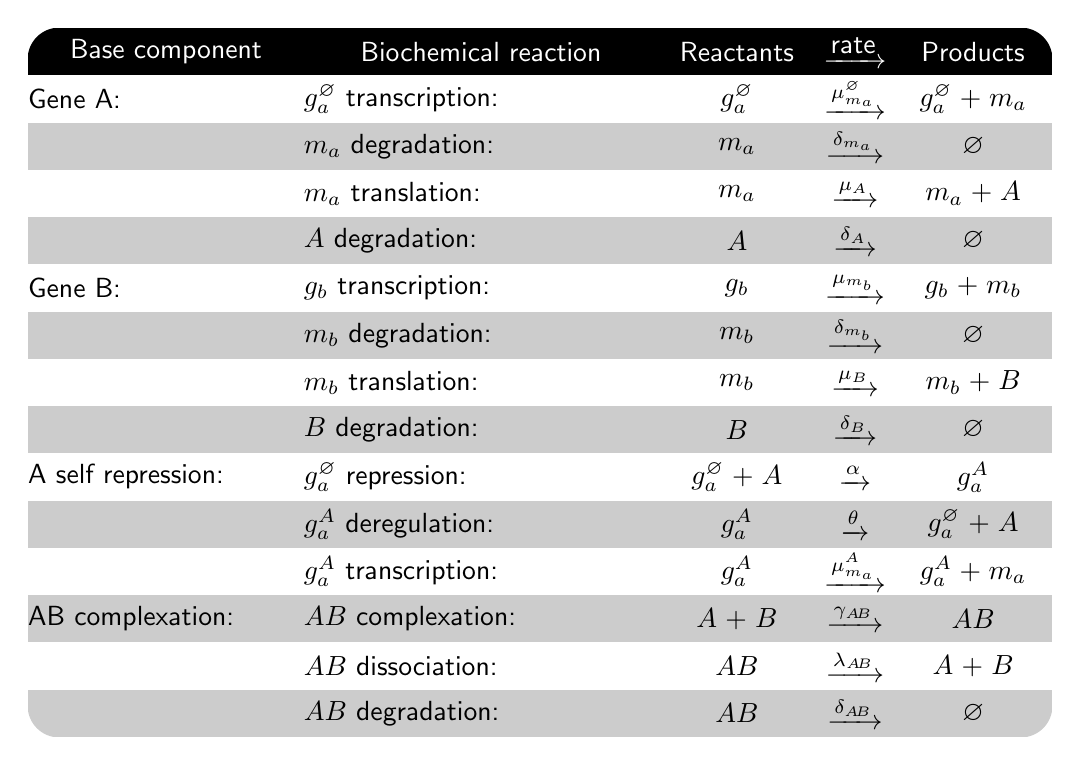
\begin{tikzpicture}
\clip node (m) [matrix,matrix of nodes,
fill=black!20,inner sep=0pt,
nodes in empty cells,
nodes={minimum height=0.6cm,minimum width=0 .5cm,anchor=center,outer sep=0,font=\sffamily},
row 1/.style={align=center,nodes={fill=black,text=white}},
column 1/.style={text width=3.5cm,align=left,every even row/.style={nodes={fill=white}}},
column 2/.style={text width=4.5cm,align=left,every even row/.style={nodes={fill=white}}},
column 3/.style={text width=2cm,align=center,every even row/.style={nodes={fill=white}}},
column 4/.style={text width=1cm,align=center,every even row/.style={nodes={fill=white}}},
column 5/.style={text width=2cm,align=center,every even row/.style={nodes={fill=white}}},
prefix after command={[rounded corners=4mm] (m.north east) rectangle (m.south west)}
] {
Base component    & Biochemical reaction           & Reactants           &$\xrightarrow{\mbox{rate}}$    & Products               \\
Gene A:      &$g_a^\varnothing$ transcription:&$g_a^\varnothing$&$\xrightarrow{\mu_{m_a}^\varnothing}$   &$g_a^\varnothing + m_a$ \\
                  &$m_a$             degradation:  &$m_a$                &$\xrightarrow{\delta_{m_a}}$   &$\varnothing$           \\
                  &$m_a$             translation:  &$m_a$                &$\xrightarrow{\mu_A}$          &$m_a + A$               \\
                  &$A$               degradation:  &$A$                  &$\xrightarrow{\delta_A}$       &$\varnothing$           \\
Gene B:           &$g_b$             transcription:&$g_b$                &$\xrightarrow{\mu_{m_b}}$      &$g_b + m_b$             \\
                  &$m_b$             degradation:  &$m_b$                &$\xrightarrow{\delta_{m_b}}$   &$\varnothing$           \\
                  &$m_b$             translation:  &$m_b$                &$\xrightarrow{\mu_B}$          &$m_b + B$               \\
                  &$B$               degradation:  &$B$                  &$\xrightarrow{\delta_B}$       &$\varnothing$           \\
A self repression:&$g_a^\varnothing$ repression:   &$g_a^\varnothing + A$&$\xrightarrow{\alpha}$         &$g_a^A$                 \\
                  &$g_a^A$           deregulation: &$g_a^A$              &$\xrightarrow{\theta}$         &$g_a^\varnothing + A$   \\
                  &$g_a^A$           transcription:&$g_a^A$              &$\xrightarrow{\mu_{m_a}^A}$    &$g_a^A + m_a$           \\
AB complexation:  &$AB$              complexation: &$A + B$              &$\xrightarrow{\gamma_{A\! B}}$&$AB$                    \\
                  &$AB$              dissociation: &$AB$                 &$\xrightarrow{\lambda_{A\! B}}$ &$A + B$                 \\
                  &$AB$              degradation:  &$AB$                 &$\xrightarrow{\delta_{A\! B}}$ &$\varnothing$           \\
};
\end{tikzpicture}
\caption{List of all the biochemical reactions which define the HAL module. By convention rates are denoted by: $\mu$ for production rates, $\delta$ for degradation rates, $\alpha$ for binding rates, $\theta$ for unbinding rates, $\gamma$ for complexation rates and $\lambda$ for dissociation rates.}
\label{BiochemicalReactions}
\end{figure}

\subsection{The complete set of differential equations}

\p Translation of the list of biochemical reactions to a set of differential equations leads to the following equations:

\begin{eqnarray}
\left\{ 
\begin{array}{ccccccccc}
\vspace{2mm}
\frac{d[g_a^\varnothing]}{dt}&=&\theta [g_A^A]                         &-&\alpha [g_a^\varnothing] [A]                      \\
\vspace{2mm}
\frac{d[m_A]}{dt}            &=&\mu_{m_A}^\varnothing [g_a^\varnothing]&+&\mu_{m_A}^A [g_A^{A}]  &-& \delta_{m_A} [m_A]     \\
\vspace{2mm}
\frac{d[A]}{dt}              &=&\mu_{A} [m_A]           &-&\gamma_{A\! B} [A][B] &+& \lambda_{A\! B} [A\! B] &-& \delta_A [A]\\
\vspace{2mm}
\frac{d[g_b^\varnothing]}{dt}&=&0                                                                                           \\
\vspace{2mm}
\frac{d[m_B]}{dt}            &=&\mu_{m_B} [g_b^\varnothing]            &-&\delta_{m_B} [m_B]                                \\
\vspace{2mm}
\frac{d[B]}{dt}              &=&\mu_{B} [m_B]          &-&\gamma_{A\! B} [A][B] &+& \lambda_{A\! B} [A\! B] &-& \delta_B [B]\\
\vspace{2mm}
\frac{d[g_A^A]}{dt}          &=&\alpha [g_a^\varnothing] [A]           &-&\theta [g_A^A]                                    \\
\vspace{2mm}
\frac{d[A\! B]}{dt}          &=&\gamma_{A\! B} [A][B]                 &-& \lambda_{A\! B} [A\! B] &-& \delta_{A\! B} [A\! B]
\end{array}
\right.
\end{eqnarray}

\section{Simplifying the equations}

\p A number of things can be done to simplify the equations without any loss of generality:

\begin{itemize}
\item Conservation of gene number $[g_A^A] + [g_a^\varnothing] = 1$ gives: $[g_A^A] = 1 - [g_a^\varnothing]$
\item Solving $\frac{d[g_b^\varnothing]}{dt}=0$ with $[g_b^\varnothing](t=0)=1$ gives: $[g_b^\varnothing]=1$
\item Solving $\frac{d[m_B]}{dt}=\mu_{m_B}-\delta_{m_B} [m_B]$ gives: $[m_B] = \frac{\mu_{m_B}}{\delta_{m_B}}$ for $t\rightarrow\infty$
\item Elimination of the $[A\! B]$ equation is possible since it does not feedback into the system.
\item Seen no confusion is possible any-more $[g_a^\varnothing]$ can be replaced by $[g]$
\item Seen no confusion is possible any-more $[m_A]$ can be replaced by $[m]$
\item $\mu_{B}\frac{\mu_{m_B}}{\delta_{m_B}}$ can be replaced by $\mu_{B}$. Where $\mu_{B}$ is not any-more the production rate of protein $B$ per $m_{B}$ per unit of time, but is now the production rate of protein $B$ per unit of time given the equillibrium distribution of $m_{B}$ is maintained.
\end{itemize}

\begin{eqnarray}
\left\{ 
\begin{array}{ccccccccc}
\vspace{2mm}
\frac{d[g]}{dt}     &=&\theta (1-[g])             &-&\alpha [g] [A]                                                      \\
\vspace{2mm}
\frac{d[m]}{dt}     &=&\mu_m^\varnothing[g]       &+&\mu_m^A(1-[g])          &-&\delta_m[m  ]                            \\
\vspace{2mm}
\frac{d[A]}{dt}     &=&\mu_A [m]                  &-&\gamma_{A\! B} [A][B]   &+&\lambda_{A\! B} [A\! B] &-& \delta_A [A] \\
\vspace{2mm}
\frac{d[B]}{dt}     &=&\mu_B                      &-&\gamma_{A\! B} [A][B]   &+&\lambda_{A\! B} [A\! B] &-& \delta_B [B] \\
\vspace{2mm}
\frac{d[A\! B]}{dt} &=&\gamma_{A\! B} [A][B]      &-&\lambda_{A\! B} [A\! B] &-&\delta_{A\! B} [A\! B]
\end{array}
\right.
\end{eqnarray}

\section{CubeSampling and PCA}

\p Since Sampling of the full parameter space was not biologically relevant and sampling of the full biologically relevant space did not give a clear result, we moved onto sampling of the neighbourhood of a point in the biologically relevant space.

\p I will deliberately not show hour previous results here (where beta correlates well to the period), since the new analysis comes before those results in the work flow. And while the PCA analysis was inspired by my knowledge of the existence of beta, the analysis is know capable of predicting beta.

\newpage

\p The PCA analysis goes as follows:

\begin{enumerate}
\item sample N ($\pm 1000$) points uniformly in a 12-D hypercube of size S\footnote{if $\overrightarrow{x}$ is a point in an M dimensional space, then an M dimensional hypercube of size S around $\overrightarrow{x}$ is defined {\bf here} as $\{\overrightarrow{y}|\forall i \in 1...M], y(i) \in [x(i)/S,x(i)*S]\}$} (2) of the parameter space around $k_{basis}$\footnote{$k_{basis}=[\theta=0.01, \delta_m=0.05, \mu_m^\varnothing=2, \mu_A=25, \mu_B=100, \gamma_{A\! B}=1000, \alpha=0.01, \mu_m^A=0.001, \delta_A=0.001, \delta_B=0.001, \delta_{A\! B}=1, \lambda_{A\! B}=0.001]$}
\item measure the period for each point and normalize it with $\delta_m$\footnote{This is necessary, since the analysis only works if the period are measured in a similar scale, but has to be analysed more thoroughly to generalize it to any system.} (remove the non oscillatory points)
\item optional?: normalize each set of parameters and the set of all the measured periods\footnote{make their average=0 and std=1}
\item merge the parameters and the period into one 13\footnote{12 parameters + the period} by N matrix, which I will call "the data matrix".
\item calculate the covariance\footnote{$cov(A)_{i,j}=\frac{1}{N-1}\sum_{k=1}^N (A_{i,k}-<A_{i,*}>)(A_{j,k}-<A_{j,*}>)$ where $<X_{i,*}>$ is the average of the i-th row of matrix X} of this data matrix
\item Calculate the smallest(???) eigenvalue of the covariance matrix and it's eigenvector, multiply both and call the result $n$.
\end{enumerate}

\p Following this process we get:

% \theta \delta_m \mu_m^\varnothing \mu_A \mu_B \gamma_{A\! B} \alpha \mu_m^A \delta_A \delta_B \delta_{A\! B} \lambda_{A\! B}

\begin{tabular}{>{$}c<{$}>{$}c<{$}>{$}c<{$}}
n(\theta)=0.0100 & n(\delta_m)=-0.0207 & n(\mu_m^\varnothing)=0.0102 \\
n(\mu_A)=0.0102 & n(\mu_B)=-0.0092 & n(\gamma_{A\! B})=0.0003 \\
n(\alpha)=-0.0004 & n(\mu_m^A)=0.0005 & n(\delta_A)=-0.0004 \\
n(\delta_B)=0.0001 & n(\delta_{A\! B})=-0.0003 & n(\lambda_{A\! B})=-0.0004 \\
\end{tabular}

\p Consider now that $\beta=\frac{\theta\mu_m^\varnothing\mu_A}{\mu_B\delta_m^2}$ and consider with $P = (\prod_k k^{n(k)})^c$ with $c=100$. Can this be a coincidence?

\newpage

\p Even better lets plot the normalized period towards P:

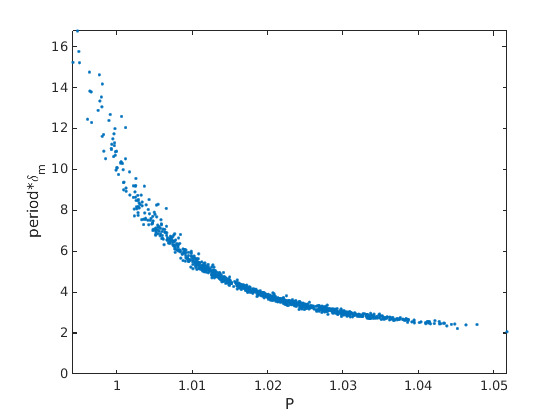
\includegraphics[width=\textwidth]{PCA_result.png}

\newpage

\section{Questions to be resolved}

\p From most to least important:

\begin{enumerate}
\item Why the smallest eigenvalue? Or is it?
\item Explain more clearly why scale with $\delta_m$ and generalize this part of the process
\item Find the name/literature of this analysis\footnote{I can not believe this has not been done before, this is a combination of 2 trivial extensions of PCA. 1) PCA on log scales 2) PCA on input/output data. However I do not even know the name of each extension separately.} (and streamline it to the standards of the field)
\item Understand the literature on non-linear PCA (and use it to perfect this technique)
\item Try with MFL (or other models)
\item Try without the log ($T=c\sum_k n(k)k$ instead of $T=(\prod_k k^{n(k)})^c$)
\item Predict c in $T=(\prod_k k^{n(k)})^c$
\item Try with an arbitrary data point (this one was known to be better then average)
\item Try without simplifying the equations ($n(\mu_B)=-1$ should be replaced by $\{n(\mu_{B}\footnotemark)=-1, n(\mu_{m_B})=-1, n(\delta_{m_B})=1\}$
\footnotetext{This is not exactly the same $\mu_{B}$}
\item Find a standardized mathematical definition of log based hypercubes
\item Check without normalizing parameters and period
\end{enumerate}

\end{document}